
\section{棋盘覆盖}
\label{sec:board-coverage}

\begin{example}\label{ex:8-8-board}
  如图$8\times8$的棋盘去掉两个角,能否用若干个$1\times2$的长方形正好覆盖?正好覆盖是指$1\times2$的长方形之间没有重叠,且所有长方形覆盖的图形与需要被覆盖的图形一致。

  \centering
  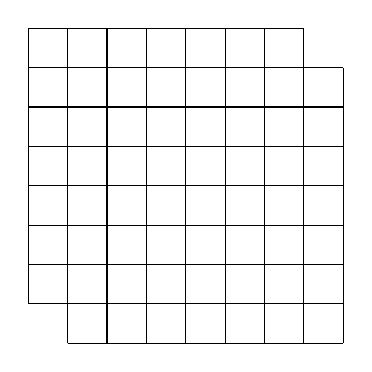
\begin{tikzpicture}[scale=.5]
    \draw(1,0)grid(7,8);
    \draw(0,1)grid(1,8);
    \draw(7,0)grid(8,7);
  \end{tikzpicture}
\end{example}
\begin{proof}[提示]
  对棋盘染色
  \begin{center}
    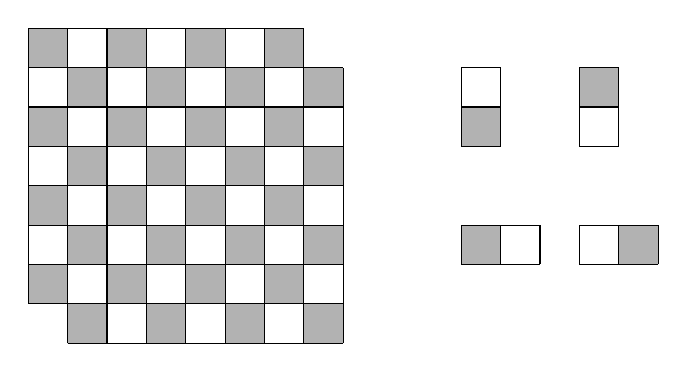
\begin{tikzpicture}[scale=.5,color=black!30,draw=black]
      \begin{scope}[shift={(0,0)}]
        \foreach \x in {1,3,5,7}{
          \fill(\x+1,0)rectangle(\x,1);
        }
        \foreach \x in{0,2,4,6}{
          \fill(\x+1,7)rectangle(\x,8);
        }
        \foreach \x in {1,3,5,7}{
          \foreach \y in {2,4,6}{
            \fill(\x+1,\y)rectangle(\x,\y+1);  
          }
        }
        \foreach \x in{0,2,4,6}{
          \foreach \y in {1,3,5,7}{
            \fill(\x+1,\y)rectangle(\x,\y+1);
          }
        }
        \draw(1,0)grid(8,1);
        \draw(0,1)grid(8,7);
        \draw(0,7)grid(7,8);
      \end{scope}
      \begin{scope}[shift={(11,2)}]
        \fill(0,0)rectangle(1,1);\draw(0,0)grid(2,1);
      \end{scope}
      \begin{scope}[shift={(14,2)}]
        \fill(2,0)rectangle(1,1);\draw(0,0)grid(2,1);
      \end{scope}
      \begin{scope}[shift={(11,5)}]
        \fill(0,0)rectangle(1,1);\draw(0,0)grid(1,2);
      \end{scope}
      \begin{scope}[shift={(14,5)}]
        \fill(0,2)rectangle(1,1);\draw(0,0)grid(1,2);
      \end{scope}
    \end{tikzpicture}
  \end{center}

  则$1\times2$的长方形覆盖住的格子只有图中4种形式,且每种形式都是覆盖一个黑格子和一个白格子。即$1\times2$的长方形能完全覆盖的形状必须黑格子数与白格子数相同。而图中的棋盘白格子比黑格子显然要少两个,所以无法用$1\times2$的长方形完全覆盖该棋盘。
\end{proof}

% \begin{example}
%   如例~\ref{ex:8-8-board},$8\times8$的棋盘能否去掉一个黑格子和一个白格子,使得剩余的$62$个格子能被$1\times2$的长方形完全覆盖?
% \end{example}

\begin{example}
  去掉一个格子的$8\times8$棋盘,能否用$1\times3$的长方形完全覆盖?

  \centering
  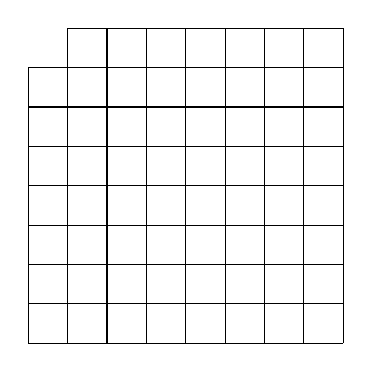
\begin{tikzpicture}[scale=.5]
    \draw(1,7)grid(8,8);
    \draw(0,0)grid(8,7);
  \end{tikzpicture}
\end{example}
\begin{proof}[提示]
  用以下方式对棋盘染色
  \begin{center}
    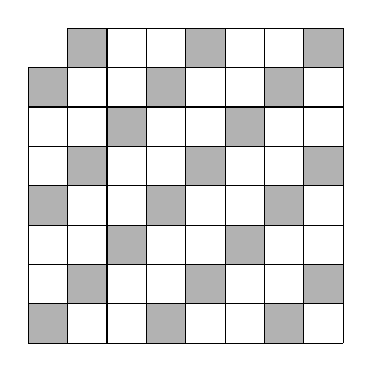
\begin{tikzpicture}[scale=.5,color=black!30,draw=black]
      \begin{scope}[shift={(0,0)}]
        \foreach \x in {0,3,6}{
          \foreach \y in {0,3,6}{
            \fill(\x+1,\y)rectangle(\x,\y+1);
          }
        }
        \foreach \x in{1,4,7}{
          \foreach \y in{1,4,7}{
            \fill(\x+1,\y)rectangle(\x,\y+1);
          }
        }
        \foreach \x in {2,5}{
          \foreach \y in {2,5}{
            \fill(\x+1,\y)rectangle(\x,\y+1);  
          }
        }
        \draw(1,7)grid(8,8);
        \draw(0,0)grid(8,7);
      \end{scope}
    \end{tikzpicture}
  \end{center}
  那么$1\times3$的长方形无论如何摆放总是覆盖一个黑格子两个白格子。
\end{proof}